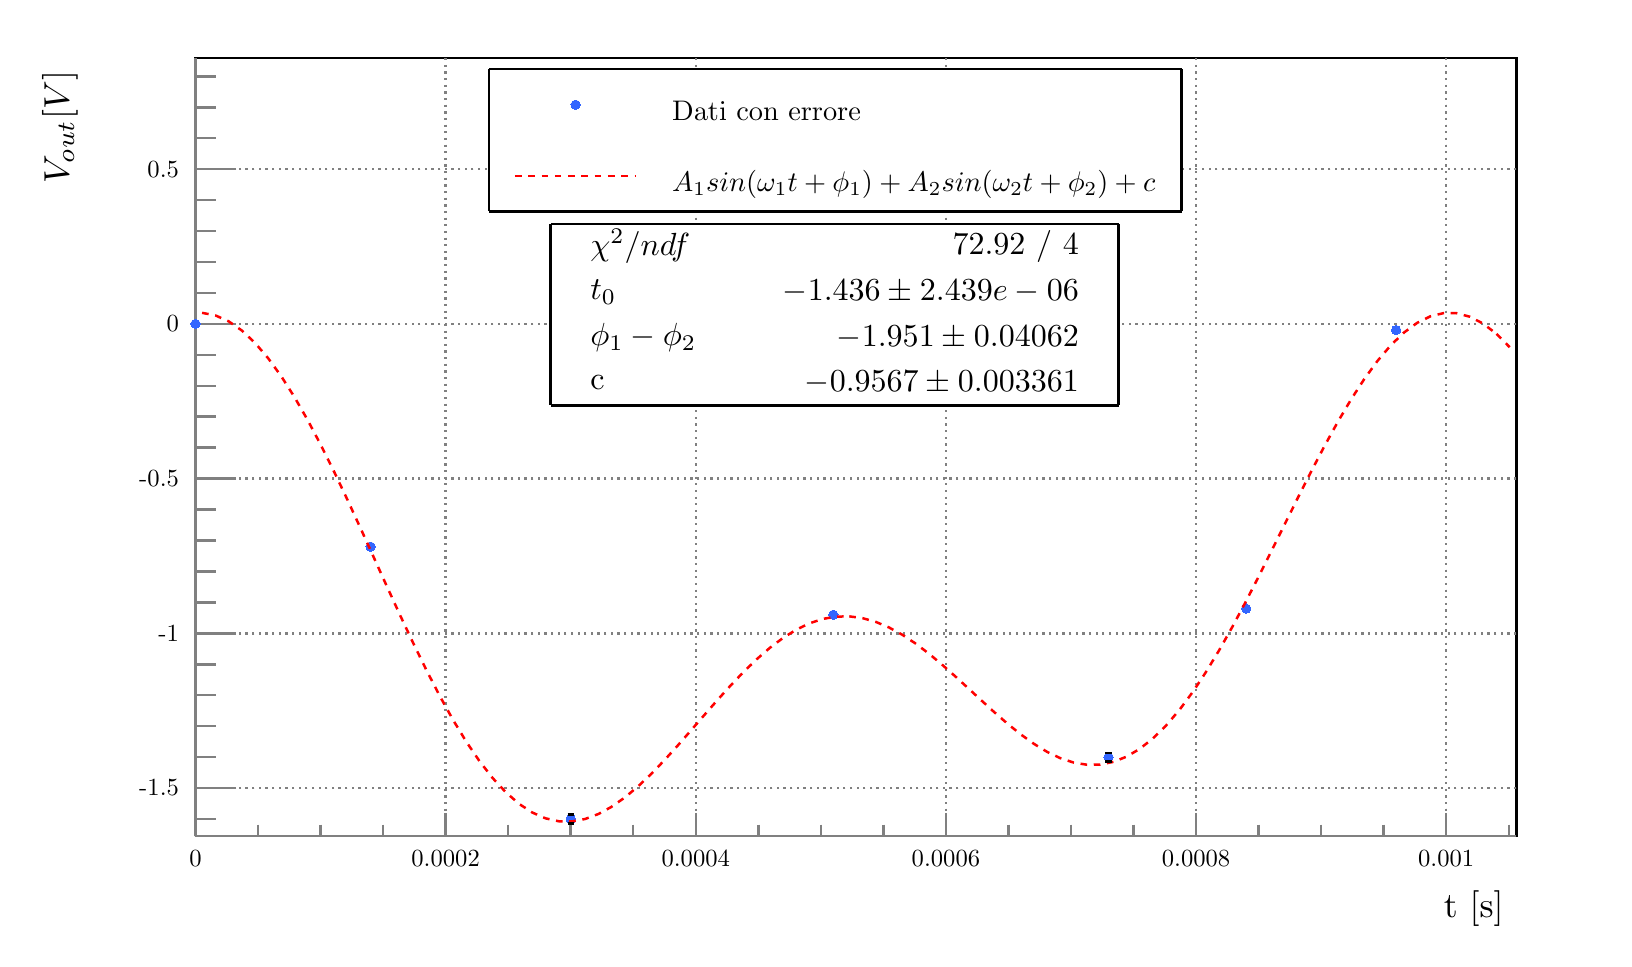
\begin{tikzpicture}
\pgfdeclareplotmark{cross} {
\pgfpathmoveto{\pgfpoint{-0.3\pgfplotmarksize}{\pgfplotmarksize}}
\pgfpathlineto{\pgfpoint{+0.3\pgfplotmarksize}{\pgfplotmarksize}}
\pgfpathlineto{\pgfpoint{+0.3\pgfplotmarksize}{0.3\pgfplotmarksize}}
\pgfpathlineto{\pgfpoint{+1\pgfplotmarksize}{0.3\pgfplotmarksize}}
\pgfpathlineto{\pgfpoint{+1\pgfplotmarksize}{-0.3\pgfplotmarksize}}
\pgfpathlineto{\pgfpoint{+0.3\pgfplotmarksize}{-0.3\pgfplotmarksize}}
\pgfpathlineto{\pgfpoint{+0.3\pgfplotmarksize}{-1.\pgfplotmarksize}}
\pgfpathlineto{\pgfpoint{-0.3\pgfplotmarksize}{-1.\pgfplotmarksize}}
\pgfpathlineto{\pgfpoint{-0.3\pgfplotmarksize}{-0.3\pgfplotmarksize}}
\pgfpathlineto{\pgfpoint{-1.\pgfplotmarksize}{-0.3\pgfplotmarksize}}
\pgfpathlineto{\pgfpoint{-1.\pgfplotmarksize}{0.3\pgfplotmarksize}}
\pgfpathlineto{\pgfpoint{-0.3\pgfplotmarksize}{0.3\pgfplotmarksize}}
\pgfpathclose
\pgfusepathqstroke
}
\pgfdeclareplotmark{cross*} {
\pgfpathmoveto{\pgfpoint{-0.3\pgfplotmarksize}{\pgfplotmarksize}}
\pgfpathlineto{\pgfpoint{+0.3\pgfplotmarksize}{\pgfplotmarksize}}
\pgfpathlineto{\pgfpoint{+0.3\pgfplotmarksize}{0.3\pgfplotmarksize}}
\pgfpathlineto{\pgfpoint{+1\pgfplotmarksize}{0.3\pgfplotmarksize}}
\pgfpathlineto{\pgfpoint{+1\pgfplotmarksize}{-0.3\pgfplotmarksize}}
\pgfpathlineto{\pgfpoint{+0.3\pgfplotmarksize}{-0.3\pgfplotmarksize}}
\pgfpathlineto{\pgfpoint{+0.3\pgfplotmarksize}{-1.\pgfplotmarksize}}
\pgfpathlineto{\pgfpoint{-0.3\pgfplotmarksize}{-1.\pgfplotmarksize}}
\pgfpathlineto{\pgfpoint{-0.3\pgfplotmarksize}{-0.3\pgfplotmarksize}}
\pgfpathlineto{\pgfpoint{-1.\pgfplotmarksize}{-0.3\pgfplotmarksize}}
\pgfpathlineto{\pgfpoint{-1.\pgfplotmarksize}{0.3\pgfplotmarksize}}
\pgfpathlineto{\pgfpoint{-0.3\pgfplotmarksize}{0.3\pgfplotmarksize}}
\pgfpathclose
\pgfusepathqfillstroke
}
\pgfdeclareplotmark{newstar} {
\pgfpathmoveto{\pgfqpoint{0pt}{\pgfplotmarksize}}
\pgfpathlineto{\pgfqpointpolar{44}{0.5\pgfplotmarksize}}
\pgfpathlineto{\pgfqpointpolar{18}{\pgfplotmarksize}}
\pgfpathlineto{\pgfqpointpolar{-20}{0.5\pgfplotmarksize}}
\pgfpathlineto{\pgfqpointpolar{-54}{\pgfplotmarksize}}
\pgfpathlineto{\pgfqpointpolar{-90}{0.5\pgfplotmarksize}}
\pgfpathlineto{\pgfqpointpolar{234}{\pgfplotmarksize}}
\pgfpathlineto{\pgfqpointpolar{198}{0.5\pgfplotmarksize}}
\pgfpathlineto{\pgfqpointpolar{162}{\pgfplotmarksize}}
\pgfpathlineto{\pgfqpointpolar{134}{0.5\pgfplotmarksize}}
\pgfpathclose
\pgfusepathqstroke
}
\pgfdeclareplotmark{newstar*} {
\pgfpathmoveto{\pgfqpoint{0pt}{\pgfplotmarksize}}
\pgfpathlineto{\pgfqpointpolar{44}{0.5\pgfplotmarksize}}
\pgfpathlineto{\pgfqpointpolar{18}{\pgfplotmarksize}}
\pgfpathlineto{\pgfqpointpolar{-20}{0.5\pgfplotmarksize}}
\pgfpathlineto{\pgfqpointpolar{-54}{\pgfplotmarksize}}
\pgfpathlineto{\pgfqpointpolar{-90}{0.5\pgfplotmarksize}}
\pgfpathlineto{\pgfqpointpolar{234}{\pgfplotmarksize}}
\pgfpathlineto{\pgfqpointpolar{198}{0.5\pgfplotmarksize}}
\pgfpathlineto{\pgfqpointpolar{162}{\pgfplotmarksize}}
\pgfpathlineto{\pgfqpointpolar{134}{0.5\pgfplotmarksize}}
\pgfpathclose
\pgfusepathqfillstroke
}
\definecolor{c}{rgb}{1,1,1};
\draw [color=c, fill=c] (0,0) rectangle (20,11.523);
\draw [color=c, fill=c] (2.12425,1.26253) rectangle (18.8978,11.1423);
\definecolor{c}{rgb}{0,0,0};
\draw [c,line width=0.9] (2.12425,1.26253) -- (2.12425,11.1423) -- (18.8978,11.1423) -- (18.8978,1.26253) -- (2.12425,1.26253);
\definecolor{c}{rgb}{1,1,1};
\draw [color=c, fill=c] (2.12425,1.26253) rectangle (18.8978,11.1423);
\definecolor{c}{rgb}{0,0,0};
\draw [c,line width=0.9] (2.12425,1.26253) -- (2.12425,11.1423) -- (18.8978,11.1423) -- (18.8978,1.26253) -- (2.12425,1.26253);
\definecolor{c}{rgb}{0.5,0.5,0.5};
\draw [c,line width=0.9] (2.12425,1.26253) -- (18.8978,1.26253);
\draw [c,dash pattern=on 0.80pt off 1.60pt ,line width=0.9] (2.12425,11.1423) -- (2.12425,1.26253);
\draw [c,dash pattern=on 0.80pt off 1.60pt ,line width=0.9] (5.30106,11.1423) -- (5.30106,1.26253);
\draw [c,dash pattern=on 0.80pt off 1.60pt ,line width=0.9] (8.47787,11.1423) -- (8.47787,1.26253);
\draw [c,dash pattern=on 0.80pt off 1.60pt ,line width=0.9] (11.6547,11.1423) -- (11.6547,1.26253);
\draw [c,dash pattern=on 0.80pt off 1.60pt ,line width=0.9] (14.8315,11.1423) -- (14.8315,1.26253);
\draw [c,dash pattern=on 0.80pt off 1.60pt ,line width=0.9] (18.0083,11.1423) -- (18.0083,1.26253);
\draw [c,dash pattern=on 0.80pt off 1.60pt ,line width=0.9] (18.0083,11.1423) -- (18.0083,1.26253);
\draw [c,line width=0.9] (2.12425,1.26253) -- (2.12425,11.1423);
\draw [c,dash pattern=on 0.80pt off 1.60pt ,line width=0.9] (18.8978,1.87346) -- (2.12425,1.87346);
\draw [c,dash pattern=on 0.80pt off 1.60pt ,line width=0.9] (18.8978,3.8383) -- (2.12425,3.8383);
\draw [c,dash pattern=on 0.80pt off 1.60pt ,line width=0.9] (18.8978,5.80314) -- (2.12425,5.80314);
\draw [c,dash pattern=on 0.80pt off 1.60pt ,line width=0.9] (18.8978,7.76798) -- (2.12425,7.76798);
\draw [c,dash pattern=on 0.80pt off 1.60pt ,line width=0.9] (18.8978,9.73281) -- (2.12425,9.73281);
\draw [c,dash pattern=on 0.80pt off 1.60pt ,line width=0.9] (18.8978,1.87346) -- (2.12425,1.87346);
\draw [c,dash pattern=on 0.80pt off 1.60pt ,line width=0.9] (18.8978,9.73281) -- (2.12425,9.73281);
\draw [c,line width=0.9] (2.12425,1.26253) -- (18.8978,1.26253);
\draw [c,line width=0.9] (2.12425,1.55245) -- (2.12425,1.26253);
\draw [c,line width=0.9] (2.91845,1.40749) -- (2.91845,1.26253);
\draw [c,line width=0.9] (3.71265,1.40749) -- (3.71265,1.26253);
\draw [c,line width=0.9] (4.50685,1.40749) -- (4.50685,1.26253);
\draw [c,line width=0.9] (5.30106,1.55245) -- (5.30106,1.26253);
\draw [c,line width=0.9] (6.09526,1.40749) -- (6.09526,1.26253);
\draw [c,line width=0.9] (6.88946,1.40749) -- (6.88946,1.26253);
\draw [c,line width=0.9] (7.68366,1.40749) -- (7.68366,1.26253);
\draw [c,line width=0.9] (8.47787,1.55245) -- (8.47787,1.26253);
\draw [c,line width=0.9] (9.27207,1.40749) -- (9.27207,1.26253);
\draw [c,line width=0.9] (10.0663,1.40749) -- (10.0663,1.26253);
\draw [c,line width=0.9] (10.8605,1.40749) -- (10.8605,1.26253);
\draw [c,line width=0.9] (11.6547,1.55245) -- (11.6547,1.26253);
\draw [c,line width=0.9] (12.4489,1.40749) -- (12.4489,1.26253);
\draw [c,line width=0.9] (13.2431,1.40749) -- (13.2431,1.26253);
\draw [c,line width=0.9] (14.0373,1.40749) -- (14.0373,1.26253);
\draw [c,line width=0.9] (14.8315,1.55245) -- (14.8315,1.26253);
\draw [c,line width=0.9] (15.6257,1.40749) -- (15.6257,1.26253);
\draw [c,line width=0.9] (16.4199,1.40749) -- (16.4199,1.26253);
\draw [c,line width=0.9] (17.2141,1.40749) -- (17.2141,1.26253);
\draw [c,line width=0.9] (18.0083,1.55245) -- (18.0083,1.26253);
\draw [c,line width=0.9] (18.0083,1.55245) -- (18.0083,1.26253);
\draw [c,line width=0.9] (18.8025,1.40749) -- (18.8025,1.26253);
\definecolor{c}{rgb}{0,0,0};
\draw [anchor=base] (2.12425,0.882265) node[scale=0.890168, color=c, rotate=0]{0};
\draw [anchor=base] (5.30106,0.882265) node[scale=0.890168, color=c, rotate=0]{0.0002};
\draw [anchor=base] (8.47787,0.882265) node[scale=0.890168, color=c, rotate=0]{0.0004};
\draw [anchor=base] (11.6547,0.882265) node[scale=0.890168, color=c, rotate=0]{0.0006};
\draw [anchor=base] (14.8315,0.882265) node[scale=0.890168, color=c, rotate=0]{0.0008};
\draw [anchor=base] (18.0083,0.882265) node[scale=0.890168, color=c, rotate=0]{0.001};
\draw [anchor= east] (18.8978,0.340681) node[scale=1.29074, color=c, rotate=0]{t [s]};
\definecolor{c}{rgb}{0.5,0.5,0.5};
\draw [c,line width=0.9] (2.12425,1.26253) -- (2.12425,11.1423);
\draw [c,line width=0.9] (2.63868,1.87346) -- (2.12425,1.87346);
\draw [c,line width=0.9] (2.38147,2.26643) -- (2.12425,2.26643);
\draw [c,line width=0.9] (2.38147,2.6594) -- (2.12425,2.6594);
\draw [c,line width=0.9] (2.38147,3.05237) -- (2.12425,3.05237);
\draw [c,line width=0.9] (2.38147,3.44533) -- (2.12425,3.44533);
\draw [c,line width=0.9] (2.63868,3.8383) -- (2.12425,3.8383);
\draw [c,line width=0.9] (2.38147,4.23127) -- (2.12425,4.23127);
\draw [c,line width=0.9] (2.38147,4.62424) -- (2.12425,4.62424);
\draw [c,line width=0.9] (2.38147,5.0172) -- (2.12425,5.0172);
\draw [c,line width=0.9] (2.38147,5.41017) -- (2.12425,5.41017);
\draw [c,line width=0.9] (2.63868,5.80314) -- (2.12425,5.80314);
\draw [c,line width=0.9] (2.38147,6.19611) -- (2.12425,6.19611);
\draw [c,line width=0.9] (2.38147,6.58907) -- (2.12425,6.58907);
\draw [c,line width=0.9] (2.38147,6.98204) -- (2.12425,6.98204);
\draw [c,line width=0.9] (2.38147,7.37501) -- (2.12425,7.37501);
\draw [c,line width=0.9] (2.63868,7.76798) -- (2.12425,7.76798);
\draw [c,line width=0.9] (2.38147,8.16094) -- (2.12425,8.16094);
\draw [c,line width=0.9] (2.38147,8.55391) -- (2.12425,8.55391);
\draw [c,line width=0.9] (2.38147,8.94688) -- (2.12425,8.94688);
\draw [c,line width=0.9] (2.38147,9.33985) -- (2.12425,9.33985);
\draw [c,line width=0.9] (2.63868,9.73281) -- (2.12425,9.73281);
\draw [c,line width=0.9] (2.63868,1.87346) -- (2.12425,1.87346);
\draw [c,line width=0.9] (2.38147,1.4805) -- (2.12425,1.4805);
\draw [c,line width=0.9] (2.63868,9.73281) -- (2.12425,9.73281);
\draw [c,line width=0.9] (2.38147,10.1258) -- (2.12425,10.1258);
\draw [c,line width=0.9] (2.38147,10.5187) -- (2.12425,10.5187);
\draw [c,line width=0.9] (2.38147,10.9117) -- (2.12425,10.9117);
\definecolor{c}{rgb}{0,0,0};
\draw [anchor= east] (2.02425,1.87346) node[scale=0.890168, color=c, rotate=0]{-1.5};
\draw [anchor= east] (2.02425,3.8383) node[scale=0.890168, color=c, rotate=0]{-1};
\draw [anchor= east] (2.02425,5.80314) node[scale=0.890168, color=c, rotate=0]{-0.5};
\draw [anchor= east] (2.02425,7.76798) node[scale=0.890168, color=c, rotate=0]{0};
\draw [anchor= east] (2.02425,9.73281) node[scale=0.890168, color=c, rotate=0]{0.5};
\draw [anchor= east] (0.402806,11.1423) node[scale=1.29074, color=c, rotate=90]{$V_{out} [V]$};
\definecolor{c}{rgb}{0.2,0.4,1};
\foreach \P in {(2.12425,7.76798), (4.34801,4.93861), (6.88946,1.4805), (10.2251,4.07408), (13.7196,2.26643), (15.4668,4.15267), (17.3729,7.68938)}{\draw[mark options={color=c,fill=c},mark size=1.681682pt, line width=0.000000pt, mark=*] plot
 coordinates {\P};}
\definecolor{c}{rgb}{1,0,0};
\draw [c,dash pattern=on 2.40pt off 2.40pt ,line width=0.9] (2.20812,7.90836) -- (2.37585,7.87642) -- (2.54359,7.80166) -- (2.71132,7.68493) -- (2.87906,7.52774) -- (3.04679,7.33216) -- (3.21453,7.10086) -- (3.38226,6.83705) -- (3.55,6.54438) --
 (3.71774,6.22695) -- (3.88547,5.88918) -- (4.05321,5.53579) -- (4.22094,5.17167) -- (4.38868,4.80186) -- (4.55641,4.43141) -- (4.72415,4.06533) -- (4.89188,3.70851) -- (5.05962,3.36562) -- (5.22735,3.04106) -- (5.39509,2.73885) -- (5.56283,2.46263)
 -- (5.73056,2.21554) -- (5.8983,2.00021) -- (6.06603,1.8187) -- (6.23377,1.67251) -- (6.4015,1.56249) -- (6.56924,1.48892) -- (6.73697,1.45144) -- (6.90471,1.44909) -- (7.07244,1.48035) -- (7.24018,1.54315) -- (7.40792,1.63493) -- (7.57565,1.75268)
 -- (7.74339,1.89299) -- (7.91112,2.05216) -- (8.07886,2.2262) -- (8.24659,2.41098) -- (8.41433,2.60224) -- (8.58206,2.79573) -- (8.7498,2.98723) -- (8.91753,3.17269) -- (9.08527,3.34825) -- (9.25301,3.51034) -- (9.42074,3.65574) -- (9.58848,3.78162)
 -- (9.75621,3.88562) -- (9.92395,3.96587) -- (10.0917,4.02106) -- (10.2594,4.05039) -- (10.4272,4.05366);
\draw [c,dash pattern=on 2.40pt off 2.40pt ,line width=0.9] (10.4272,4.05366) -- (10.5949,4.03122) -- (10.7626,3.98399) -- (10.9304,3.91345) -- (11.0981,3.82156) -- (11.2658,3.71079) -- (11.4336,3.58401) -- (11.6013,3.44449) -- (11.769,3.2958) --
 (11.9368,3.14175) -- (12.1045,2.98634) -- (12.2722,2.83366) -- (12.44,2.6878) -- (12.6077,2.55282) -- (12.7755,2.43263) -- (12.9432,2.33093) -- (13.1109,2.25113) -- (13.2787,2.19628) -- (13.4464,2.16905) -- (13.6141,2.17161) -- (13.7819,2.20564) --
 (13.9496,2.27224) -- (14.1173,2.37198) -- (14.2851,2.50478) -- (14.4528,2.67002) -- (14.6205,2.86642) -- (14.7883,3.09218) -- (14.956,3.34489) -- (15.1237,3.62166) -- (15.2915,3.91909) -- (15.4592,4.23339) -- (15.627,4.56036) -- (15.7947,4.89555) --
 (15.9624,5.23425) -- (16.1302,5.57164) -- (16.2979,5.90281) -- (16.4656,6.22286) -- (16.6334,6.527) -- (16.8011,6.81063) -- (16.9688,7.06938) -- (17.1366,7.29923) -- (17.3043,7.49655) -- (17.472,7.65817) -- (17.6398,7.78144) -- (17.8075,7.86426) --
 (17.9753,7.90515) -- (18.143,7.90323) -- (18.3107,7.85826) -- (18.4785,7.77066) -- (18.6462,7.64149);
\draw [c,dash pattern=on 2.40pt off 2.40pt ,line width=0.9] (18.6462,7.64149) -- (18.8139,7.47241);
\definecolor{c}{rgb}{1,1,1};
\draw [color=c, fill=c] (6.63327,6.73347) rectangle (13.8477,9.03808);
\definecolor{c}{rgb}{0,0,0};
\draw [c,line width=0.9] (6.63327,6.73347) -- (13.8477,6.73347);
\draw [c,line width=0.9] (13.8477,6.73347) -- (13.8477,9.03808);
\draw [c,line width=0.9] (13.8477,9.03808) -- (6.63327,9.03808);
\draw [c,line width=0.9] (6.63327,9.03808) -- (6.63327,6.73347);
\draw [anchor= west] (6.99399,8.75) node[scale=1.15722, color=c, rotate=0]{$\chi^{2} / ndf $};
\draw [anchor= east] (13.487,8.75) node[scale=1.15722, color=c, rotate=0]{ 72.92 / 4};
\draw [anchor= west] (6.99399,8.17385) node[scale=1.15722, color=c, rotate=0]{$t_{0}    $};
\draw [anchor= east] (13.487,8.17385) node[scale=1.15722, color=c, rotate=0]{$ -1.436 \pm 2.439e-06$};
\draw [anchor= west] (6.99399,7.5977) node[scale=1.15722, color=c, rotate=0]{$\phi_{1} - \phi_{2} $};
\draw [anchor= east] (13.487,7.5977) node[scale=1.15722, color=c, rotate=0]{$ -1.951 \pm 0.04062$};
\draw [anchor= west] (6.99399,7.02154) node[scale=1.15722, color=c, rotate=0]{c        };
\draw [anchor= east] (13.487,7.02154) node[scale=1.15722, color=c, rotate=0]{$ -0.9567 \pm 0.003361$};
\draw [c,line width=0.9] (6.88946,1.52058) -- (6.88946,1.53983);
\draw [c,line width=0.9] (6.84938,1.53983) -- (6.92954,1.53983);
\draw [c,line width=0.9] (6.88946,1.44042) -- (6.88946,1.42116);
\draw [c,line width=0.9] (6.84938,1.42116) -- (6.92954,1.42116);
\draw [c,line width=0.9] (13.7196,2.30651) -- (13.7196,2.31959);
\draw [c,line width=0.9] (13.6795,2.31959) -- (13.7597,2.31959);
\draw [c,line width=0.9] (13.7196,2.22635) -- (13.7196,2.21327);
\draw [c,line width=0.9] (13.6795,2.21327) -- (13.7597,2.21327);
\definecolor{c}{rgb}{1,1,1};
\draw [color=c, fill=c] (6.63327,6.73347) rectangle (13.8477,9.03808);
\definecolor{c}{rgb}{0,0,0};
\draw [c,line width=0.9] (6.63327,6.73347) -- (13.8477,6.73347);
\draw [c,line width=0.9] (13.8477,6.73347) -- (13.8477,9.03808);
\draw [c,line width=0.9] (13.8477,9.03808) -- (6.63327,9.03808);
\draw [c,line width=0.9] (6.63327,9.03808) -- (6.63327,6.73347);
\draw [anchor= west] (6.99399,8.75) node[scale=1.15722, color=c, rotate=0]{$\chi^{2} / ndf $};
\draw [anchor= east] (13.487,8.75) node[scale=1.15722, color=c, rotate=0]{ 72.92 / 4};
\draw [anchor= west] (6.99399,8.17385) node[scale=1.15722, color=c, rotate=0]{$t_{0}    $};
\draw [anchor= east] (13.487,8.17385) node[scale=1.15722, color=c, rotate=0]{$ -1.436 \pm 2.439e-06$};
\draw [anchor= west] (6.99399,7.5977) node[scale=1.15722, color=c, rotate=0]{$\phi_{1} - \phi_{2} $};
\draw [anchor= east] (13.487,7.5977) node[scale=1.15722, color=c, rotate=0]{$ -1.951 \pm 0.04062$};
\draw [anchor= west] (6.99399,7.02154) node[scale=1.15722, color=c, rotate=0]{c        };
\draw [anchor= east] (13.487,7.02154) node[scale=1.15722, color=c, rotate=0]{$ -0.9567 \pm 0.003361$};
\definecolor{c}{rgb}{1,1,1};
\draw [color=c, fill=c] (5.8517,9.1984) rectangle (14.6493,11.002);
\definecolor{c}{rgb}{0,0,0};
\draw [c,line width=0.9] (5.8517,9.1984) -- (14.6493,9.1984);
\draw [c,line width=0.9] (14.6493,9.1984) -- (14.6493,11.002);
\draw [c,line width=0.9] (14.6493,11.002) -- (5.8517,11.002);
\draw [c,line width=0.9] (5.8517,11.002) -- (5.8517,9.1984);
\draw [anchor=base west] (8.0511,10.3482) node[scale=1.02369, color=c, rotate=0]{Dati con errore};
\definecolor{c}{rgb}{0.2,0.4,1};
\foreach \P in {(6.9514,10.5511)}{\draw[mark options={color=c,fill=c},mark size=1.681682pt, line width=0.000000pt, mark=*] plot coordinates {\P};}
\definecolor{c}{rgb}{0,0,0};
\draw [anchor=base west] (8.0511,9.44639) node[scale=1.02369, color=c, rotate=0]{$A_{1}sin(\omega_{1} t + \phi_{1})+A_{2}sin(\omega_{2} t + \phi_{2}) + c$};
\definecolor{c}{rgb}{1,0,0};
\draw [c,dash pattern=on 2.40pt off 2.40pt ,line width=0.9] (6.18161,9.6493) -- (7.72119,9.6493);
\end{tikzpicture}
